\documentclass{article}
\usepackage{tikz} 
\usepackage[utf8]{inputenc}
\usepackage{amsmath}
\usepackage{listings}
\usepackage{amsfonts}
\usepackage{amssymb}
\usepackage{tabularx}
\usepackage{enumitem}
\usepackage{algorithm}% http://ctan.org/pkg/algorithm
\usepackage[noend]{algpseudocode}% http://ctan.org/pkg/algorithmicx
\usepackage[margin=0.7in]{geometry}
\usepackage{tikz}

\usepackage{graphicx}
\usetikzlibrary{arrows,positioning} 
\usepackage{subcaption}
\thispagestyle{empty}
\usepackage{multicol,caption}
\pgfarrowsdeclarecombine{ring}{ring}{}{}{o}{o}

\DeclareMathOperator{\ringarrow}{\raisebox{0.5ex}{\tikz[baseline]{\draw[ring->](0,0)--(2em,0);}}}

\tikzset{
    %Define standard arrow tip
    >=stealth',
    %Define style for boxes
    observed/.style={
           rectangle,
           rounded corners,
           draw=black, thick,
           minimum width=6em,
           minimum height=2.2em,
           font=\footnotesize,
           text centered,
           },
     latent/.style={
           circle,
           rounded corners,
           draw=black, thick, dashed,
           minimum width=2.2em,
           minimum height=2.2em,
           font=\footnotesize,
           text centered,
           fill=black!10!white
           },
    % Define arrow style
    pil/.style={
           o->,
           thick,
           shorten <=2pt,
           shorten >=2pt,},
    sh/.style={ shade, shading=axis, left color=red, right color=green,
    shading angle=45 }
    
}
   
\begin{document}
%
\def\ci{\perp\!\!\!\perp} % from Wikipedia


\begin{figure}
\centering
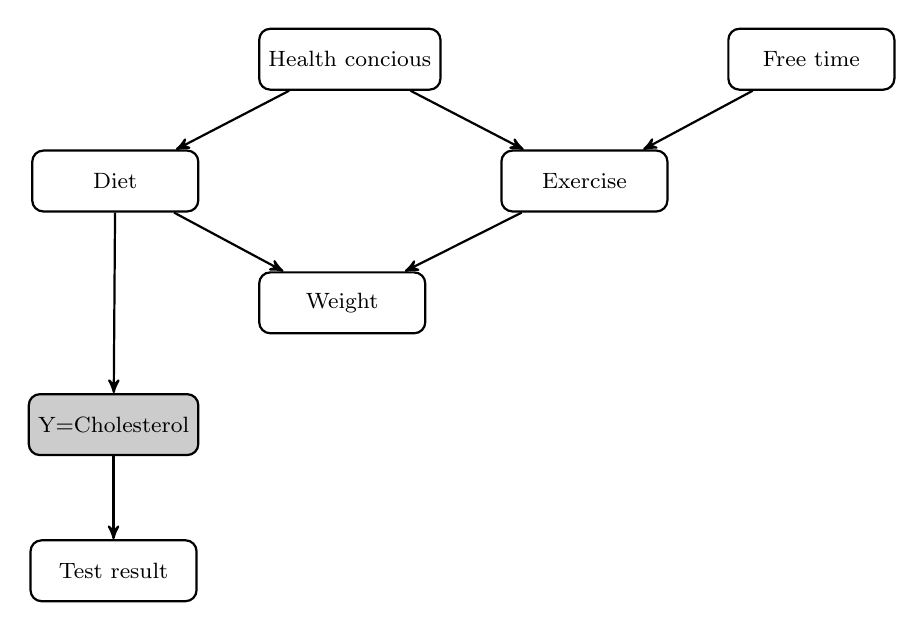
\begin{tikzpicture}[->,shorten >=0pt,shorten <=0pt,node distance=3em,thick,main node/.style={observed}, lt/.style={latent}]
\node[main node](1){Health concious};
\node[main node, below left=of 1](2){Diet};
\node[main node, below right=of 1](3){Exercise};
\node[main node, below right=of 2](4){Weight};
\node[main node, fill=black!20!white,below left=of 4](5){Y=Cholesterol};
\node[main node, below =of 5](6){Test result};
\node[main node, above right=of 3](7){Free time};
\path[]
	(1) edge (2) edge (3)
	(2) edge (4) edge (5)
	(3) edge (4)
	(5) edge (6)
	(7) edge (3);
\end{tikzpicture}
\end{figure}

\end{document}
